\chapter{Speaker Recognition Systems}
\label{ch:speaker-recognition-system}

The process of voice recognition lies on the field of pattern classification, with the speaker and his or her utterance (a speech signal) as inputs for a classifier and a decision as output. This decision may be, given an utterance $\boldsymbol{Y}$ produced by a speaker $\mathcal{S}$ and a set $\boldsymbol{\mathcal{S}} = \{\mathcal{S}_1, ..., \mathcal{S}_S\}$ of known users,

\begin{equation}
    \mathcal{S} \gets \mathcal{S}_i \text{, if } i = \arg\max_j P(\mathcal{S}_j|\boldsymbol{Y}).
    \label{eq:decision_speaker_identification}
\end{equation}

\noindent This is a case of speaker identification and the output is a $\mathcal{S}_i$ from $\boldsymbol{\mathcal{S}}$. Another type of decision is

\begin{equation}
    \text{if } P(\mathcal{S}_i|\boldsymbol{Y}) \verifytest{\alpha}{\mathcal{S}}
    \label{eq:decision_speaker_verification}
\end{equation}

\noindent This is a speaker verification decision, with a binary output, given a $\mathcal{S}$ who produced $\boldsymbol{Y}$, a claimed identity $\mathcal{S}_i$ from $\boldsymbol{\mathcal{S}}$ and a threshold of acceptance $\alpha$. This chapter (and indirectly the whole document) is about the type of decision seen in \equationref{decision_speaker_verification}.

\section{Basic Concepts}

\subsection{Utterance}

An utterance is a piece of speech produced by a speaker. It may be a word, a statement or any vocal sound. The terms \emph{utterance} and \emph{speech signal} sometimes are used interchangeably, but here speech signal will be associated to an utterance recorded, digitalized and ready to be processed. An example is shown in \figureref{speech_signal}.

\begin{figure}[ht]
    \centering
    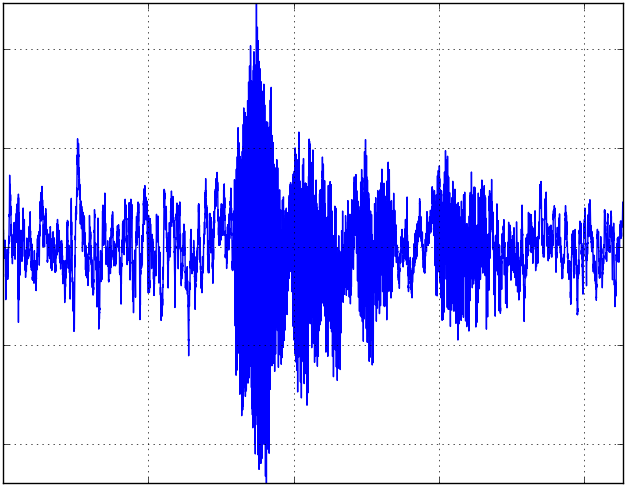
\includegraphics[width=\textwidth]{speech_signal}
    \caption{Speech signal for utterance ``karen livescu" \cite{woo.park.hazen.2006}.}
    \label{fig:speech_signal}
\end{figure}

\subsection{Features}

The raw speech signal is unfit for usage by a recognition system. For a correct processing, the unique features from the speaker's vocal tract are extracted, reducing the number of variables the system needs to deal with (leading to a simpler implementation) and performing a better evaluation (and avoiding the curse of dimensionality). This extraction is executed by the MFCC algorithm, explained in \chapterref{feature-extraction}. Due to the stationary properties of the speech signal when analyzed in a short period of time, it is divided in overlapping frames of small and predefined length, to avoid ``loss of significancy" in the features \cite{davis.mermelstein.1980, rabiner.schafer.2007}.

\subsection{Dependency x Independency}

When designing a speaker recognition system, one of the most important aspects to consider is the type of text dependency it will have. In a text-dependent system the choice of what to say is made at design time, with different degrees of freedom. The testing utterance must be a subset of the training set. A simpler version may require that the same text be spoken during the model's training and testing phases, while a more sophisticated one may allow the speaker to say just a few words from a sentence or even speak them out of order. The most common acoustic model used for this system is the HMM, with the unit modeled and the number of states depending heavily on the type of application \cite{hebert.2008}.

\begin{figure}[ht]
    \centering
    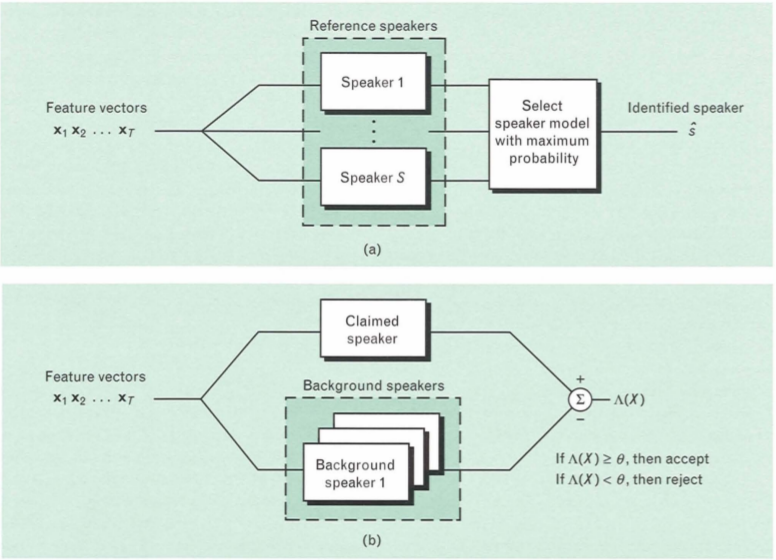
\includegraphics[width=\textwidth]{speaker-recognition-2}
    \caption{Speaker-recognition systems for identification and verification \cite{reynolds.1995}.}
    \label{fig:speaker-recognition-2}
\end{figure}

Text-independent recognition is less problematic than the previous one for several reasons. First, the designer does not need to worry about what the speaker will say, since it is a vocal sound. The recognition is performed around the unique features of each vocal tract, shown when the person speaks. Second, for being free of time constraints, a HMM of single state (i.e. a GMM) fits well for the task \cite{hebert.2008}. Third, the ability to apply text-independent verification to unconstrained speech encourages the use of audio recorded from a wide variety of sources (e.g., speaker indexing of broadcast audio or forensic matching of law-enforcement microphone recordings) \cite{reynolds.campbell.2008}.

As stated in \sectionref{speaker-recognition}, the focus of this paper is in text-independent speaker verification, and due to that it is necessary to understand what is the likelihood ratio test and how the models are trained and tested (more detailed in \chapterref{gmm}).

\subsection{Likelihood Ratio Test}

TODO basear-se na seção 2 do artigo ``Speaker Verification Using Adapted Gaussian Mixture Models" e na seção 38.2 de ``Text-Independent Speaker Recognition".

\section{Basic Speaker Verification Architecture}

\subsection{Training Phase}

\subsection{Test Phase}